% *==================================================================================*
% *                     Review vs. Camera-Ready settings                             *
% *==================================================================================*
%
% REVIEW: Use the following command for submitting the paper (double-blind,
% for review):
% \documentclass{Interspeech}
%
% CAMERA-READY: Use the following command for the camera-ready version, one
% affiliation per line:
\documentclass[]{Interspeech}
% *==================================================================================*


% **************************************
% *                                    *
% *      STOP !   DO NOT DELETE !      *
% *          READ THIS FIRST           *
% *                                    *
% * This template also includes        *
% * important INSTRUCTIONS that you    *
% * must follow when preparing your    *
% * paper. Read it BEFORE replacing    *
% * the content with your own work.    *
% **************************************

%==================================================================================
% Title
% Must exactly match the title entered into the paper submission system
\title{PyPhonPlan: Simulating phonetic planning with dynamic neural fields and task dynamics}

%==================================================================================
% Authors, affiliations, emails
% In camera-ready mode, these details are loaded from author-info.tex -- this has been gitignored to avoid inclusion of author information in review version, but removing author-info.tex from .gitignore will inject author information when [cameraready] flag is set to True.
\ifcameraready
    \input{author-info}
\fi

%==================================================================================

% Keywords
\keywords{computational modeling, phonetic planning, dynamic neural fields, task dynamics, speech production}




%==================================================================================
% Content

\begin{document}

\maketitle

% the abstract here must exactly match the abstract entered into the paper submission system
\begin{abstract}
    % 1000 characters. ASCII characters only. No citations.
    We introduce PyPhonPlan, a Python toolkit for implementing dynamical models of phonetic planning using coupled dynamic neural fields and task dynamic simulations. The toolkit provides modular components for defining planning, perception and memory fields, as well as between-field coupling, gestural inputs, and using field activation profiles to solve tract variable trajectories. We illustrate the toolkit's capabilities through an example application:~simulating production/perception loops with a coupled memory field, which demonstrates the framework's ability to model interactive speech dynamics using representations that are temporally-principled, neurally-grounded, and phonetically-rich. PyPhonPlan is released as open-source software and contains executable examples to promote reproducibility, extensibility, and cumulative computational development for speech communication research.
\end{abstract}




\section{Introduction}

The production of speech appears at first to be unfathomably complex. Speakers must navigate the precise temporal coordination of a high-dimensional neuromuscular space with many degrees-of-freedom, with the ultimate goal of shaping a channel of moving air to achieve meaningful action in a rich social environment. Despite this apparent complexity, there is abundant evidence across biological motor control that organisms simplify the control of high-dimensional movement by constraining it to a smaller number of functionally relevant variables \cite{bernstein1967, haken-etal1985}. In the domain of speech production, one of the most popular models of these functionally relevant variables is task dynamics \cite{fowler1980, kelso-etal1986, saltzman-munhall1989, browman-goldstein1992, byrd-saltzman1998, iskarous2017}. Task dynamics hypothesizes that an abstract dynamical force called a \textit{gesture} drives low-dimensional \textit{tract variables} that control geometric properties of the vocal tract, such as lip aperture (LA) or tongue tip constriction degree (TTCD). Tract variables are the coordinate system in which the articulatory goals of speech are defined, and are achieved by flexibly reconfiguring groups of articulators (tongue tip, lower lip, jaw) to meet the ongoing demands of speech.

A fundamental assumption in task dynamics is that tract variables are governed by point attractor dynamics, where a gesture drives a tract variable toward an equilibrium position. However, in conventional task dynamic models, these target values are stipulated as invariant parameters, with no intrinsic mechanism for learning, memory or sensory influences on speech production. A major development in this respect is the integration of dynamic neural fields (DNFs) for movement planning with task dynamic theory \cite{kirov-gafos2007, tilsen2007}. A dynamic neural field (DNF) is a low-dimensional representation of a functional neural population, which is defined over a metric variable for a sensory or movement parameter \cite{erlhagen-schoener2002, schoener-etal2016}. The field's dynamics evolve over time under the influence of sensory inputs, memory, and field-internal dynamics \cite{schutte-etal2003, schneegans-etal2016, simmering-spencer2008, spencer-etal2025}.

The last decade has witnessed an explosion of DNF models for speech planning and phonetic processes \cite{kirov-gafos2007, tilsen2007, roon-gafos2016, iskarous2016, tilsen2019, harper2021, shaw-tang2023, stern-shaw2023, kirkham-strycharczuk2024, kirkham-etal2025, chaturvedi-shaw2025}. While much of this work has focused on relatively low-level phonetic variation, there is increasing evidence that DFT can also model more traditionally `phonological' phenomena \cite{shaw2025}, as well as lexical meaning \cite{stern-pinango2026}. An excellent review of DFT models for speech communication can be found in \cite{stern2025}. In light of the current landscape, there is a need to develop modern computational frameworks that make this integration of dynamic neural fields and task dynamics accessible to a broader community. To address this gap, we introduce PyPhonPlan, a Python toolkit for simulating phonetic planning using coupled dynamic neural fields and task dynamic equations. The toolkit provides modular components for defining activation fields, coupling architectures, gestural inputs, and task dynamic simulations. This allows researchers to instantiate diverse planning architectures within a common computational framework that is tailored towards speech communication research. The major contributions of this paper are:

\begin{enumerate}
    \item We present an open-source Python toolkit for simulating phonetic planning using coupled dynamic neural fields and task dynamic equations.
    \item We advance a modular architecture that permits flexible model development, extension and customization, including multi-layer fields, coupling mechanisms, memory fields, and tract variable simulations.
    \item We release the toolkit with executable examples and code notebooks to promote reproducibility, extensibility, and cumulative computational research in speech communication.
\end{enumerate}

The software and code notebooks are available at the following GitHub repository (anonymized for peer review):~\url{https://anonymous.4open.science/r/PyPhonPlan-Interspeech26/}. The rest of this paper outlines the conceptual, mathematical and computational implementation of model components, before illustrating its functionality via a three-layer perception/planning/memory model of interactive speech.



\section{Model architecture and implementation}

In this section, we review the components of the dynamic field model implemented in PyPhonPlan. For an excellent and extensive tutorial introduction to dynamic neural fields see \cite{schoener-etal2016}.

\subsection{Field dynamics}

The dynamics of a control variable (e.g.~TTCD) can be formalized as a dynamic neural field \cite{erlhagen-schoener2002}, with activation of a neural population defined over the control variable's metric range $x$,

\begin{multline}
\tau \dot{u}(x,t) = -u(x,t) + h + s(x,t)
\\
+ \int k(x-x') g(u(x',t))dx' + q\xi(x,t)
\label{dnf}
\end{multline}


where $\tau$ dictates the rate of field evolution. $u(x,t)$ is time-dependent activation at each field site $x$, with the negative sign in (\ref{dnf}) providing stable decay towards the resting level $h$. $s(x,t)$ represents an input to the field, and $\xi(x,t)$ is Gaussian noise scaled by a coefficient $q$ \cite{schoener-etal2016}. The interaction kernel $k(x - x')$ defines excitatory and inhibitory forces across the DNF, which is explained in greater detail below. $x$ here represents a one-dimensional articulatory or acoustic variable (e.g.~TTCD, LA, $F_1$). Figure \ref{fig:dnf}  visualizes the dynamics of a single DNF, where two time-scheduled inputs at $x = -5$ and $x = +5$ drive activation above the resting level at different field locations.

\begin{figure}
  \centering
  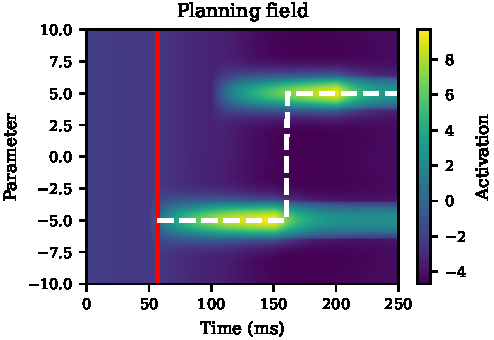
\includegraphics[width=\columnwidth]{figs/fig1a.pdf}
  \caption{Heatmap of a single-layer DNF with two competing inputs at $x = -5$ and $x = +5$. The dotted line tracks peak activation above threshold. The red line indicates the start of above-threshold activation.}
  \label{fig:dnf}
\end{figure}



\subsection{Inputs}

The field in (\ref{dnf}) has its own intrinsic dynamics, but without sensory input the field's dynamics will converge to a stable, sub-threshold resting level (see Section \ref{interactions}). Inputs to the DNF drive activation away from the resting level and excite localized areas of the field. These inputs represent task-related input (i.e.~responding to an experimental prompt), retrieval of a speech planning representation, or sensory/perceptual inputs (i.e.~hearing or shadowing another speaker). An input $s(x,t)$ is defined as a Gaussian distribution over a parameter $x$ with amplitude $a$, centroid $p$ and width $w$,

\begin{equation}
s(x,t) = \sum_{i} a_{i} \exp \left[ - \frac{(x-p_{i})^2}{2w^2_{i}} \right].
\label{dnf_input}
\end{equation}

This means that gestural inputs are inherently distributional, in contrast to the invariant target values in many task dynamic implementations. Inputs are typically time-bound; in the current implementation, timing is manually stipulated, but we discuss more principled timing mechanisms in Section \ref{discussion}.

\subsection{Field interactions and thresholds}
\label{interactions}

A key property of DNFs is that field sites interact with one another:~nearby sites excite each other while distant sites inhibit each other. This interaction profile has two key consequences:~it stabilizes peaks of activation once they form (through local self-excitation), and it enables competition between peaks, where activation of one peak will inhibit others. These dynamics are captured by the interaction kernel $k(x-x')$, which takes a `Mexican hat' profile, with local excitation $c_{\text{excite}}$ surrounded by lateral inhibition $c_{\text{inhibit}}$, plus a global inhibition term $c_{\text{global}}$:

\begin{multline}
k(x - x') = \frac{c_{\text{excite}}}{\sqrt{2 \pi \sigma_{\text{excite}}}} \exp \left[ -\frac{(x-x')^2}{2 \sigma^2_{\text{excite}}} \right] 
\\
- \frac{c_{\text{inhibit}}}{\sqrt{2 \pi \sigma_{\text{inhibit}}}} \exp \left[ -\frac{(x-x')^2}{2 \sigma^2_{\text{inhibit}}} \right] - c_{\text{global}}
\label{kernel}
\end{multline}


The interaction kernel is gated by a sigmoid function,

\begin{equation}
g(u) = \frac{1}{1+\exp (-\beta (u-\alpha))}
\label{dnf_sigmoid}
\end{equation}

where $\beta$ is the slope of the sigmoid and $\alpha$ is a threshold parameter (typically $\alpha = 0$). This ensures that only field sites with activation above $\alpha$ contribute to the interaction dynamics.


\subsection{Memory field}
\label{memory}

\begin{figure}
  \centering
  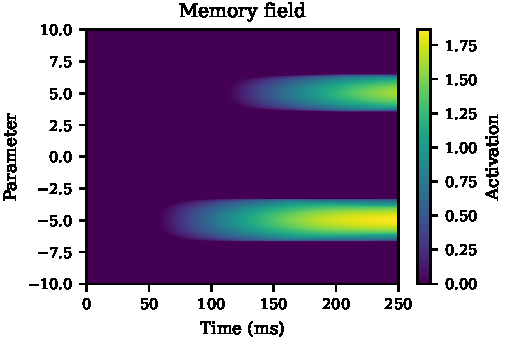
\includegraphics[width=\columnwidth]{figs/fig1b.pdf}
  \caption{Memory field coupled to the planning field in Figure~\ref{fig:dnf}. The memory trace reflects a history of above-threshold planning activation, with a broader spatial profile due to convolution with $w(x-x')$.}
  \label{fig:memory}
\end{figure}


In addition to the standard fields described above, PyPhonPlan implements memory fields (see Figure \ref{fig:memory}), which are a special kind of field coupled to the planning field that stores a history of activation traces \cite{samuelson-etal2011}. This stored history can then bias the planning field on subsequent productions. Memory dynamics are implemented as a Hebbian layer over the memory field $u_{\text{mem}}(x,t)$ in (\ref{eq:memory}) subject to local interactions $w(x-x')$.

\begin{equation}
\dot{u}_{\text{mem}}(x,t)  =
\begin{cases} 
    \frac{1}{\tau_{\text{mem}}} [-u_{\text{mem}}(x,t) \\
    + \int w(x-x') g(u(x',t)) dx'], 
    & u(x,t) > \alpha \\[0.5em]
    \frac{1}{\tau_{\text{decay}}} [-u_{\text{mem}}(x,t)], 
    & u(x,t) \leq \alpha
\end{cases}
\label{eq:memory}
\end{equation}

When the planning field  $u(x,t)$ exceeds the $\alpha$ threshold, the sigmoid $g(u)$ determines the pattern of activation that is convolved into the memory field, at a rate determined by $\tau_{\text{mem}}$. When $u(x,t) \leq \alpha$, memory decays at a rate of $\tau_{\text{decay}}$. The memory field evolves on a slower timescale  than the planning field, while memory decay is slowest, such that $\tau_{\text{decay}} > \tau_{\text{mem}} > \tau$.





\subsection{Cross-field coupling}
\label{coupling}

In multi-layer models, fields can be coupled with strength $c$, weighting the influence of perception or memory on planning. However, a strong perceptual input could push the planning field over the activation threshold, involuntarily triggering production even when no response input is present. PyPhonPlan avoids this via an (optional) latched gate on the planning field:

\begin{equation}
\gamma(t) =
\begin{cases}
    1 & \text{if } s_{\text{planning}}(x, t) > 0 \text{ for any } x, \\
    \gamma(t - \Delta t) & \text{if } u_{\text{planning}}(x, t) > \alpha \text{ for any } x, \\
    0 & \text{otherwise}
\end{cases}
\label{eq:gating}
\end{equation}

When $\gamma(t) = 0$, activation is clamped so it cannot exceed threshold $\alpha$, ensuring that coupling from perception or memory can shape sub-threshold activation but cannot initiate production without an explicit input cue. The gate opens ($\gamma = 1$) when direct input arrives to the planning field ($s_{\text{planning}}(x, t) > 0$) and holds its value ($\gamma(t - \Delta t)$) while activation is above-threshold.
  
\subsection{Task dynamics}

We integrate DNF planning dynamics with a critically-damped harmonic oscillator model \cite{saltzman-munhall1989} for the evolution of tract variables, where $m = 1$, $k$ is a constant, and $b = 2\sqrt k$,

\begin{equation}
m\ddot{x} + b\dot{x} + k(x - x^*(t)) = 0.
\end{equation}

Following \cite{tilsen2019, kirkham-strycharczuk2024, shaw2025}, we derive the tract variable's time-varying target $x^*(t)$ from the planning DNF. The spatial position $x$ corresponding to peak activation in $u$ from the planning field at each time step is taken as the planned target value. An alternative formulation is to use a single constant value for $x^*(t)$, which can be derived from identifying the parameter value that corresponds to a peak activation plateau.

\begin{equation}
x^*(t)= \arg\max_x u(x,t)
\end{equation}

In addition to the above core components, PyPhonPlan contains methods for visualization, animations, extracting DNF activation peaks, task dynamic solvers, and example simulation cases. See the GitHub repository for further information.



\section{Application: Three-layer model}

The PyPhonPlan GitHub repository contains fully-documented code notebooks for typical DNF simulation cases. In this section, we review a three-layer model of a phonetic shadowing task \cite{goldinger1998}, which couples perception, planning and memory fields, and simulates tract variables from DNF activation. Parameter values and additional information can be found in the GitHub repository at \texttt{examples/shadowing.ipynb}.


\begin{figure*}[t]
  \centering
  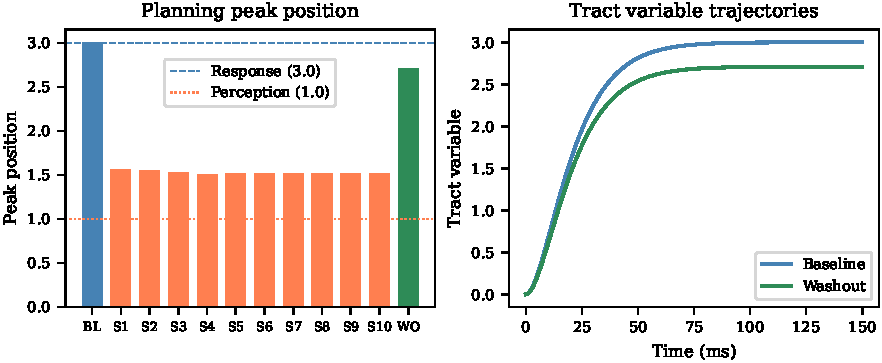
\includegraphics[width=\textwidth]{figs/fig2.pdf}
  \caption{Shadowing simulation results. Left: planning peak position across baseline with no perceptual input (BL), 10 shadowing trials with strong perceptual input (S1--S10), and washout with no perceptual input (WO). Right: tract variable trajectories for baseline versus washout, showing subtle articulatory consequences of memory-driven convergence.}
  \label{fig:sim}
\end{figure*}


\subsection{Three-layer field}

We define a three-layer architecture of perception, planning and memory fields. The perception field represents the influence of perceiving an interlocutor's speech on the speech planning field. For the sake of simplicity, we assume an arbitrary parameter space for $x \in [-10, 10]$, which is an articulatory dimension. Note that the perception field captures the influence of auditory perception on the planning field, rather than modelling the auditory-acoustic signal directly. The perception field is

\begin{multline}
\tau_{\text{perception}}\dot{u}_{\text{perception}}(x,t)  = -u_{\text{perception}}(x,t) + h + s_{\text{perception}}(x,t)
\\
+ \int z(x-x') g(u_{\text{perception}}(x',t))dx' + q\xi(x,t)
\label{eq:perception}
\end{multline}

where $z(x-x')$ is a perception-specific interaction kernel. The advantage of a separate perception field, rather than perception as a simple input to the planning field, is that it allows perception to have its own intrinsic timescale and stabilization dynamics (e.g.~competition between perceptual inputs).

The memory field is implemented exactly as described in Section \ref{memory}, so Equation (\ref{eq:memory}) is not repeated here. The speech planning field also follows the generic DNF architecture,

\begin{multline}
\tau \dot{u}(x,t) = -u(x,t) + h + c_{\text{perception}} u_{\text{perception}}(x,t)
\\
+ c_{\text{memory}} u_{\text{memory}}(x,t) + c_{\text{response}}s_{\text{response}}(x,t)
\\
+ \int k(x-x') g(u(x',t))dx' + q\xi(x,t)
\label{eq:planning}
\end{multline}

but with coupling to $u_{\text{perception}}(x,t)$ and $u_{\text{memory}}(x,t)$ with strengths $c_{\text{perception}}$ and $c_{\text{memory}}$. These weights reflect the relative strength of perception/memory coupling, such as attentional strength or socially-modulated perception. In the following example, the interaction between production/perception fields is linear and unidirectional (perception $\rightarrow$ planning). The input $s_{\text{response}}(x,t)$ is a response input, prompted by retrieving an appropriate motor plan in response to a cue to speak. The $\gamma$-gating described in Section \ref{coupling} prevents perceptual coupling from involuntarily triggering production, but residual perception activation at response onset can bias the spatial location of peak formation. The memory field coupling $u_{\text{memory}}(x,t)$ means that the current state of memory additionally influences the planning field, while the memory field is simultaneously updated as a consequence of ongoing planning dynamics.
 
 
\subsection{Simulating phonetic shadowing}

We now illustrate a full simulation of a very simple shadowing task \cite{goldinger1998}. The shadowing task paradigm is as follows:~ 

\begin{enumerate}
    \item \textbf{Baseline}:~speaker produces a word cued by an orthographic representation on a computer screen.
    \item \textbf{Shadow}:~speaker hears a (pre-recorded) talker and is prompted to repeat the word they hear.
    \item \textbf{Washout}:~speaker produces a word cued by an orthographic representation on a computer screen.
\end{enumerate}
 Speakers typically show phonetic convergence towards the interlocutor's voice during the shadowing block, with limited evidence for persistent post-shadowing convergence \cite{goldinger1998, babel2012}. In this sense, the shadowing task represents a highly artificial case of phonetic accommodation, whereby speakers adapt their speech in response to interlocutors.

The simulations in this section follow the above structure, with 1 baseline trial, 10 shadowing trials, and 1 washout trial. Note that $s_{\text{response}}(x,t)$ is the intended production and $s_{\text{perception}}(x,t)$ is the auditory prompt. During each trial, $u_{\text{memory}}(x,t)$ is updated based on the current activation profile in the planning field. This predicts that our model speaker should converge to the perceptual input token, and that the resulting memory field update should yield minor evidence of convergence in the post-shadowing washout block. In terms of timing, perception and response inputs are sequential, with the perception field's finite time constant ($\tau = 10$) providing residual bias during planning peak formation. 


\subsection{Simulation results}
Figure \ref{fig:sim} shows the simulation results. The left panel shows the location of peak activation measured during the response plateau across all trials. During baseline, the planning peak is at the response position ($x = 3.0$). During shadowing, the speaker hears the interlocutor's production that diverges from their own ($x = 1.0$). The strong attention to perceptual input shifts the planning peak toward the interlocutor ($x = 1.58$ on the first shadowing trial). The washout planning peak retains some of this convergence effect, shifting $-0.26$ units from baseline ($x = 2.74$). This shift is driven by accumulated memory traces from shadowing trials, which bias the planning field. The right panel shows the corresponding tract variable trajectories for baseline and washout trials, with targets derived from the plateau peak positions. The washout trajectory reaches a lower endpoint than baseline, demonstrating how field-level convergence propagates to articulatory output. As such, interactional phonetic phenomena emerge from the coupled dynamics of speech planning, perception and memory. 


\section{Discussion}
\label{discussion}

PyPhonPlan lowers the barrier to entry for dynamical models of phonetic planning, with a computational toolkit that is tailored to the requirements of researchers in speech communication. Importantly, this includes researchers working in different theoretical paradigms who wish to generate dynamical predictions to test against their own models. The repository contains example simulations, including single- and multi-layer field simulations, plus mapping from field dynamics to task dynamics.

Several design choices leave room for further extension. Most importantly, input timing is currently stipulated; future versions could implement coupled oscillator models \cite{nam-saltzman2003}, conditions of satisfaction for input deactivation \cite{sandamirskaya-schoner2010, chaturvedi-shaw2025b}, or competitive queuing for selection-activation dynamics \cite{tilsen2016, tilsen2022}. Additionally, the current task dynamic integration extracts time-varying targets from field peaks but lacks the full articulator-to-tract-variable mapping characteristic of standard models \cite{saltzman-munhall1989}. In terms of challenges, DNFs are inherently low-dimensional (typically 1--4 dimensions) and do not scale well to higher-dimensional fields. While this encourages an interpretable and biophysically-grounded approach, it constrains modelling of higher-dimensional problems and thus requires theoretical commitments about which control variables to model. 

A longer-term aim is to integrate PyPhonPlan with an extended Task Dynamic Application (TADA) architecture \cite{nam-etal2004}, enabling the use of gestural scores as inputs to the DNF and providing time-varying targets to the full TADA articulatory model. State feedback control is another important frontier; models such as FACTS \cite{parrell-etal2019} incorporate feedback into the task dynamic framework, while DNF \cite{chaturvedi-shaw2025} and other dynamical \cite{tilsen2022} architectures for feedback monitoring also show promise. Finally, the coupling of speaker-listener DNFs will facilitate new agent-based models of interactive speech dynamics, with the advantage of inherently dynamic and rich phonetic representations. For example, exemplar models of speech processing tend towards static phonetic representations, where memory retrieval and execution are instantaneous \cite{pierrehumbert2001}. In contrast, the DNF architecture explicitly models the dynamics of memory, perception and production, with dynamics specified at every scale.


\section{Conclusion}

In conclusion, PyPhonPlan is an open-source toolkit for building flexible models of phonetic planning using coupled dynamic neural fields and task dynamics. It provides a modular architecture that supports reproducible experimentation and transparent model development, thereby advancing a framework for cumulative computational research in speech communication.


%\section{Acknowledgments}

%XXX was funded by XXX fellowship XXX and XXX grant XXX, the latter of which was also supported by the XXX. 


\bibliographystyle{IEEEtran}
\bibliography{bibliography}

\end{document}

%%% Local Variables:
%%% mode: LaTeX
%%% TeX-master: t
%%% End:
